\appendix
\numberwithin{equation}{subsection}
\numberwithin{figure}{subsection}
\numberwithin{table}{subsection}
\section*{付録}
\addtocontents{toc}{\vspace{-10pt}}
\addcontentsline{toc}{section}{付録}

\renewcommand{\thesubsection}{\Alph{subsection}}
\subsection{2粒子ホログラムの近似}
\label{sec:appendix_2particle}
奥行方向距離を持たない近接同径粒子のホログラフィックパターン導出に際して,以下を仮定した.
\begin{equation}
    1 + 2\Re \left\{ \psi_{A_1} \overline{\psi_{A_2}} \right\} - 2\Re \left\{\overline{\psi_b}\left( \psi_{A_1} + \psi_{A_2} \right)\right\} = -1
    \tag{\ref{th:extratermsApprox}}
\end{equation}
この仮定が,2つの粒子が重複しない条件で妥当であることを示す.

まず,式(\ref{th:extratermsApprox})中の各複素振幅$\psi_{A_1}$,$\psi_{A_2}$,$\psi_{b}$は以下で与えられる.
\begin{align}
    \psi_{A_1}(x,y) &= \exp{\left(\mathrm{j}\frac{2\pi}{\lambda}z_0\right)} \left\{ 1 + \frac{\mathrm{j}}{\lambda z_0} \exp{ \left( \frac{\mathrm{j} \pi r^2}{\lambda z_0} \right)} \pi a^2 \frac{2J_1(2\pi a r/ \lambda z_0)}{2\pi a r/ \lambda z_0}  \right\} \\
    \psi_{A_2}(x,y) &= \exp{\left(\mathrm{j}\frac{2\pi}{\lambda}z_0\right)} \left\{ 1 + \frac{\mathrm{j}}{\lambda z_0} \exp{ \left( \frac{\mathrm{j} \pi r'^2}{\lambda z_0} \right)} \pi a^2 \frac{2J_1(2\pi a r'/ \lambda z_0)}{2\pi a r'/ \lambda z_0}  \right\} \\
    \psi_b(x,y) &= \exp{\left(\mathrm{j}\frac{2\pi}{\lambda}z_0\right)}
\end{align}
ただし,$r = \sqrt{x^2 + y^2}$,$r' = \sqrt{(x-\Delta \xi)^2 + (y-\Delta \eta)^2}$である.また,$z_0>0$とした.このとき,以下が成り立つ.
\begin{align}
    &1 + 2\Re \left\{ \psi_{A_1} \overline{\psi_{A_2}} \right\} - 2\Re \left\{\overline{\psi_b}\left( \psi_{A_1} + \psi_{A_2} \right)\right\} \\
    =& -1 + \frac{1}{\lambda^2 z_0^2} \cos{\left( \frac{\pi \left( r^2-r'^2 \right)}{\lambda z_0} \right) \pi^2 a^4  \frac{2J_1(2\pi a r/ \lambda z_0)}{2\pi a r/ \lambda z_0} \frac{2J_1(2\pi a r'/ \lambda z_0)}{2\pi a r'/ \lambda z_0}}
    \label{appendixEq:extraterm}
\end{align}
式(\ref{appendixEq:extraterm})の右辺第2項が十分小さければ,式(\ref{th:extratermsApprox})は成り立つ.$\Delta \xi =0$,$\Delta \eta=0$であれば,式(\ref{th:particleIrradiance})の右辺第3項と一致することに注意する.

関数$2J_1(x)/x$は$x=0$以外の点で定義されており,常に$|2J_1(x)/x| < 1$である.同様に$|\cos(x)|<1$であるから,式(\ref{appendixEq:extraterm})の右辺第2項は以下を満たす.
\begin{equation}
    -\frac{\pi^2 a^4}{\lambda^2 z_0^2} < \frac{1}{\lambda^2 z_0^2} \cos{\left( \frac{\pi \left( r^2-r'^2 \right)}{\lambda z_0} \right) \pi^2 a^4  \frac{2J_1(2\pi a r/ \lambda z_0)}{2\pi a r/ \lambda z_0} \frac{2J_1(2\pi a r'/ \lambda z_0)}{2\pi a r'/ \lambda z_0}} < \frac{\pi^2 a^4}{\lambda^2 z_0^2}
\end{equation}
無次元数$\pi^2 a^4 / \lambda^2 z_0^2$は半径$a$,粒子の伝搬距離$z_0$に顕著に依存する.ホログラム画像は\SI{8}{bit}で記録され,背景光の実振幅が画像輝度値で64程度になるようカメラの露光時間を調整するため,例えば$64\pi^2 a^4 / \lambda^2 z_0^2$が1より小さい場合は,この成分による輝度値変動はないと言える.本論文の実験条件では,粒子の平均直径が\SI{85}{\um},伝搬距離の最小値が\SI{220}{\mm},記録波長が$\lambda = \SI{632.8}{\nm}$であるから,
\begin{equation}
    \frac{64\pi^2 a^4}{\lambda^2 z_0^2} \approx 0.106
\end{equation}
となり,ホログラムの輝度値変化として記録されない.したがって,式(\ref{th:extratermsApprox})における仮定は妥当であると言える.

\subsection{異径・奥行方向距離を持つ場合の2粒子ホログラム}
\label{sec:appendix_deviation}
本論文では,記録面に対して垂直な方向,すなわち奥行方向の距離を持たない同径の近接粒子ホログラムを扱った.しかし,実際には当然奥行方向距離を有し粒子径の異なる粒子衝突が発生する.この場合,2粒子ホログラムはどのように変化するか,またこれらの条件でもスペクトル分布上の縞パターンによって近接検出が可能か調べる.

\subsubsection{奥行方向距離を持たない異径粒子組}
\label{sec:appendix_deviation_radius}
\ref{sec:twoParticleHologram}節と同様,座標原点中心の粒子1,$\psi_{A_1}$と$(\Delta \xi, \Delta \eta)$中心の粒子2,$\psi_{A_1}$について考える.粒子1の半径を$a_1$,粒子2の半径を$a_2 = a_1 + \Delta a$とする.これらについて,式(\ref{th:fourierOfA}),(\ref{th:particle1Fourier}),(\ref{th:particle2Fourier})より以下が成り立つ.
\begin{gather}
    \varphi_{A_1} (\alpha,\beta) = \mathcal{F} \left\{ \left|\psi_{A_1}\right|^2 \right\} = \cos{\left( \pi \lambda z_0 \gamma^2 \right)} \tilde{A}(\alpha,\beta;a_1) \\
    \varphi_{A_1} (\alpha,\beta) = \mathcal{F} \left\{ \left|\psi_{A_2}\right|^2 \right\} = \cos{ \left( \pi \lambda z_0 \gamma^2 \right) } \exp{\left( -2\pi \mathrm{j}\left( \alpha \Delta \xi + \beta \Delta \eta \right) \right)} \tilde{A}(\alpha,\beta;a_2) \\
    \tilde{A}(\alpha,\beta;a) = \mathcal{F}\left\{ A \right\} = \pi a^2 \frac{2J_1(2\pi a \gamma)}{2\pi a \gamma}
\end{gather}
したがって,原点以外におけるホログラムのフーリエ変換$\varphi(\alpha,\beta)$は以下で与えられる.
\begin{align}
    \varphi(\alpha,\beta) &= \varphi_{A_1}(\alpha,\beta) + \varphi_{A_2}(\alpha,\beta) \\
    &= \cos{\left( \pi \lambda z_0 \gamma^2 \right)} \left\{ \tilde{A}(\alpha,\beta;a_1) + \exp{\left( -2\pi \mathrm{j}\left( \alpha \Delta \xi + \beta \Delta \eta \right) \right)} \tilde{A}(\alpha,\beta;a_2) \right\}
\end{align}
スペクトル分布$S = |\varphi|^2$は以下のように計算できる.
\begin{align}
    S &= \left| \varphi(\alpha,\beta) \right|^2 \\
    &= \cos^2{\left( \pi \lambda z_0 \gamma^2 \right)} \left| \tilde{A}(\alpha,\beta;a_1) + \exp{\left( -2\pi \mathrm{j}\left( \alpha \Delta \xi + \beta \Delta \eta \right) \right)} \tilde{A}(\alpha,\beta;a_2) \right|^2 \\
    &= \cos^2{\left( \pi \lambda z_0 \gamma^2 \right)} \left\{ \tilde{A}_1^2+\tilde{A}_2^2 + 2\tilde{A}_1^2\tilde{A}_2^2 \cos{\left( 2\pi \left( \alpha \Delta \xi + \beta \Delta \eta \right) \right)} \right\}
    \label{appendixEq:diffdiamspec}
\end{align}
ただし,$\tilde{A}_1 = \tilde{A}(\alpha,\beta;a_1)$,$\tilde{A}_2 = \tilde{A}(\alpha,\beta;a_2)$とした.

$\tilde{A}_2$が以下の形で表されるとする.
\begin{gather}
    \tilde{A}_2 = \tilde{A}_1 + O(\gamma) \\
    O(\gamma) = (a+ \Delta a) \frac{J_1(2\pi (a + \Delta a) \gamma)}{\gamma} - a \frac{J_1(2\pi a \gamma)}{\gamma}
\end{gather}
このとき,式(\ref{appendixEq:diffdiamspec})は以下のようにも表せる.
\begin{equation}
    \frac{S}{4\cos^2{\left( \pi \lambda z_0 \gamma^2 \right)}} = \tilde{A}^2_1 \cos^2{\left( \pi \left( \alpha \Delta \xi + \beta \Delta \eta \right) \right)} +  \tilde{A}_1 O \cos^2{\left( \pi \left( \alpha \Delta \xi + \beta \Delta \eta \right) \right)} + O^2
    \label{appendixEq:residual}
\end{equation}
$O(\gamma)$は定義により動径$\gamma = \sqrt{\alpha^2 + \beta^2}$に依存する関数である.したがって,近接粒子組の半径が異なる場合もスペクトル分布上の縞パターン形状には影響を与えない.

\subsubsection{奥行方向距離を持つ同径粒子組}
\label{sec:appendix_deviation_z}

ここでも,座標原点中心の粒子1,$\psi_{A_1}$と$(\Delta \xi, \Delta \eta)$中心の粒子2,$\psi_{A_1}$について考える.粒子1の$z$軸座標を$z = 0$,粒子1と粒子2の奥行方向距離を$\Delta \zeta$とし,粒子1が粒子2よりも記録面に近い位置にあることとすると,記録面$z = z_1$における複素振幅$\psi(x,y;z_1)$は以下のように計算できる.
\begin{align}
    \psi(x,y; z = 0 - \delta z) &=  \mathcal{F}^{-1} \left\{ \mathcal{F}\left\{1 - A(x-\Delta \xi,y- \Delta \eta)\right\} \cdot G_{\Delta \zeta} \right\} \\
    \psi(x,y) &= \mathcal{F}^{-1} \left\{ \mathcal{F}\left\{ \psi(x,y;z = 0-\delta z) \cdot \left( 1 - A(x,y) \right) \right\} \cdot G_{z_1} \right\}
\end{align}
ここで,$G_z$は距離$z$の光伝播をあらわす角スペクトル法の伝搬関数である.粒子1と2の平面内距離が十分大きい場合は記録面の複素振幅は各粒子の物体光の和で表現できるが,今回のような近接条件では上式の計算が必要であり,またこの式の理論的な計算は困難である.そこで,本節では数値計算と実験によって$\Delta \zeta$とスペクトル分布上縞パターンの関係をみる.

ホログラムの数値生成及び実験による記録条件をTable \ref{table:appendixBcondition}に示す.また,実験装置の概要図をFig. \ref{fig:appendixBsetup}に示す.この実験装置は,Fig. \ref{fig:stripePatternExperiment}に示す装置から,マイクロメータによるガラスプレートの移動方向を$z$軸方向に変更したものである.

Fig. \ref{fig:appendixBresult}に,数値計算と実験それぞれによって得られたホログラムとそのスペクトル分布の例を示す.この例の奥行方向距離は$z=0$である.数値生成したホログラム,実験によって得たホログラムともに同様のパターンが記録されスペクトル上の縞パターンが得られていることがわかる.ここで得たスペクトル分布と,各$\Delta \zeta$におけるスペクトル分布の相互相関を計算したプロットをFig. \ref{fig:appendixBcorrelation}に示す.この相互相関は,$\Delta \zeta$が大きくなるにつれて減少していることがわかる.これは,$\Delta \zeta$が大きくなるにつれて,スペクトル分布の縞パターンが淡くなり確認が困難になるためである.数値計算・実験結果ともに相関係数の減少傾向は一致していることがわかる.それぞれのバイアスは異なるが,これは実験結果のスペクトル分布においてはもとのホログラムの背景ノイズによる高周波成分があるためである.

ホログラムの光伝播による像再生では,粒子像は奥行方向に$\Delta L \approx 4a^2/\lambda$ 程度の伸びを有することが知られている.本節における条件では伸び長さは$\Delta L \approx \SI{100}{\mm}$程度となるが,マイクロメータの可動域限界によりこの範囲までの計測は行えていない.今後は粒子伸び長さと粒子奥行方向距離に対する縞パターンの検出可能性を定量する必要がある.

\begin{table}[H]
    \centering
    \caption{Numerical generation and experimental recording conditions of holograms for $\Delta \zeta$ dependence experiment.}
    \label{table:appendixBcondition}
    \begin{tabular}{lll}
    Quantity                               & Value                                             & Unit     \\ \hline \hline
    Dot diameter $2a$                      & 250                                               & \si{\um} \\ \hline
    Dot distance in $x$-axis $\Delta \xi$  & 420                                               & \si{\um} \\ \hline
    Dot distance in $y$-axis $\Delta \eta$ & 50                                                & \si{\um} \\ \hline 
    Dot distance in $z$-axis $\Delta \zeta$& 0 to 3000 (numerical simulation)                  & \si{\mm} \\ 
                                           & 0 to 2780 in every 50 (experiment)                & \si{\mm} \\ \hline 
    Recorded wavelength $\lambda$          & 632.8                                             & \si{\nm} \\ \hline
    Propagated distance $z_0$              & 220                                               & \si{\mm} \\ \hline
    Pixel pitch of hologram $\Delta x$     & 10                                                & \si{\um}
    \end{tabular}
\end{table}


\begin{figure}[H]
    \centering
    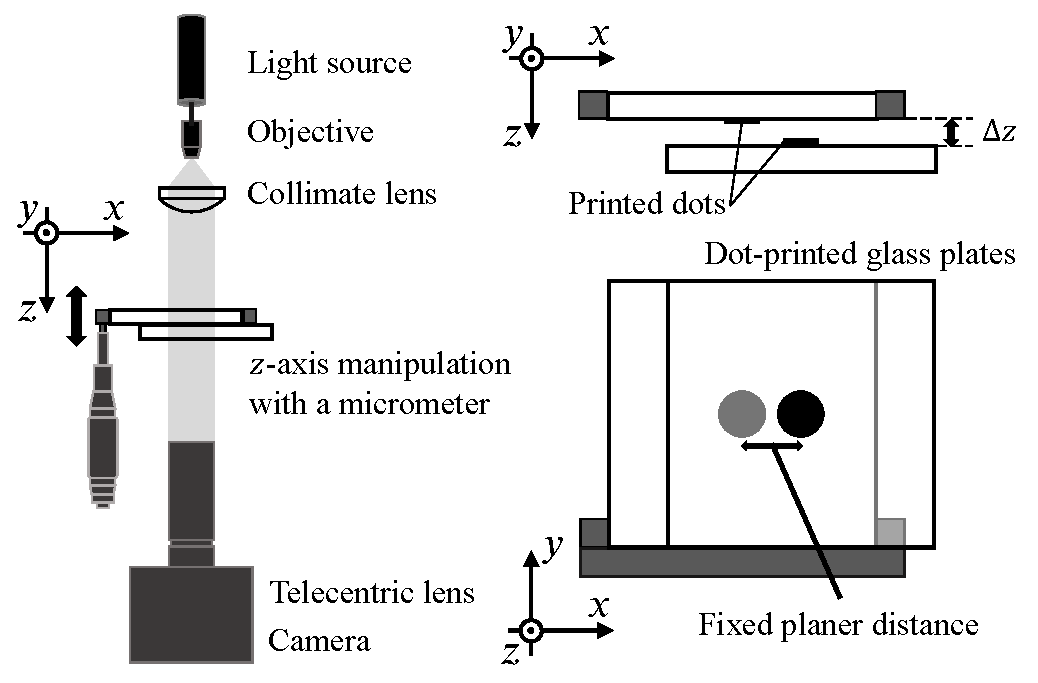
\includegraphics[width=0.8\linewidth]{./Figure/7_Appendix/expdiagram.pdf}
    \caption{Schematic diagram of experimental setup. The $z$-axis distance between dots is varied by manipulating one of the two glass plates with dots printed on them with a micrometer. The planer distance between the two glass plates is fixed at $\Delta \xi = \SI{420}{\um}$,$\Delta \eta = \SI{50}{\um}$.}
    \label{fig:appendixBsetup}
\end{figure}


\begin{figure}[H]
    \centering
    \begin{subfigure}[t]{0.45\linewidth}
        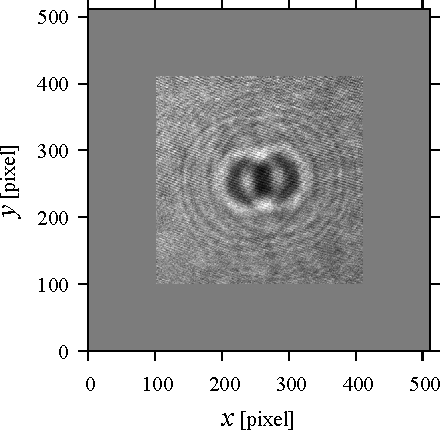
\includegraphics[width=\linewidth]{./Figure/7_Appendix/data/holoexp.pdf}
        \caption{Positive hologram}
        \label{fig:appendixBresult:expholo}
    \end{subfigure}
    \hfill
    \begin{subfigure}[t]{0.45\linewidth}
        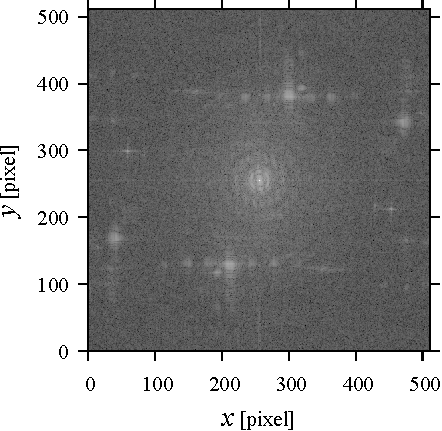
\includegraphics[width=\linewidth]{./Figure/7_Appendix/data/fftexp.pdf}
        \caption{Negative hologram}
        \label{fig:appendixBresult:expfft}
    \end{subfigure}

    \begin{subfigure}[t]{0.45\linewidth}
        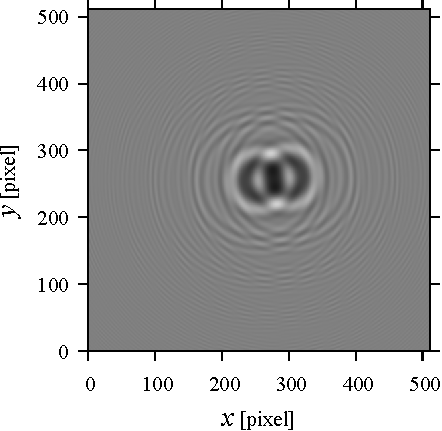
\includegraphics[width=\linewidth]{./Figure/7_Appendix/data/holonum.pdf}
        \caption{Positive hologram spectrum}
        \label{fig:appendixBresult:numholo}
    \end{subfigure}
    \hfill
    \begin{subfigure}[t]{0.45\linewidth}
        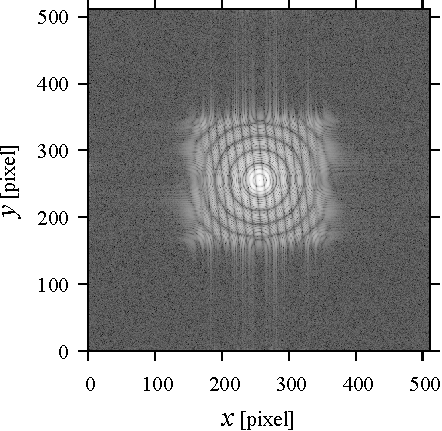
\includegraphics[width=\linewidth]{./Figure/7_Appendix/data/fftnum.pdf}
        \caption{Negative hologram spectrum}
        \label{fig:appendixBresult:numfft}
    \end{subfigure}

    \caption{Example of recorded holograms and their spectra. The holograms are recorded at $\Delta \zeta = \SI{0}{\mm}$. The experimental hologram is cropped at the center so that the target fringe pattern is visible.} 
    \label{fig:appendixBresult}
\end{figure}

\begin{figure}[H]
    \centering
    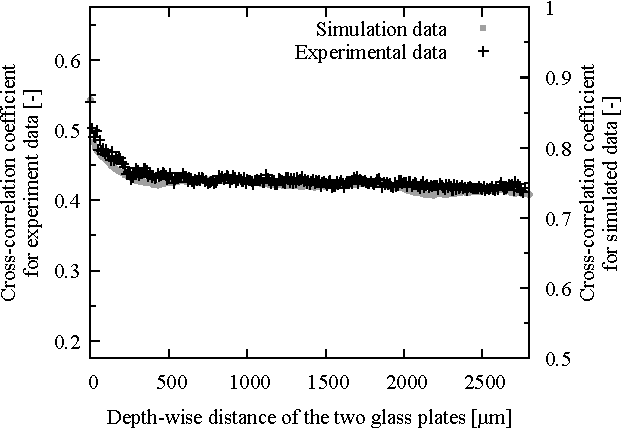
\includegraphics[width=0.8\linewidth]{./Figure/7_Appendix/result.pdf}
    \caption{Cross-correlation between the spectrum of the hologram recorded at $\Delta \zeta = \SI{0}{\mm}$ and the spectra of the holograms recorded at $\Delta \zeta$. The range of $\Delta \zeta$ is given in Table \ref{table:appendixBcondition}.}
    \label{fig:appendixBcorrelation}
\end{figure}
